\section{Resultados y discusión}

\subsection{Experimentos de captura de protocolos}

El objetivo de este experimento fue modelar el tráfico de la red como una fuente de información cuyos símbolos son los protocolos que están contenidos dentro de los paquetes Ethernet, a la que llamamos $S$.

\subsubsection{Laboratorio de universidad}

\begin{figure}[H]
	\centering
	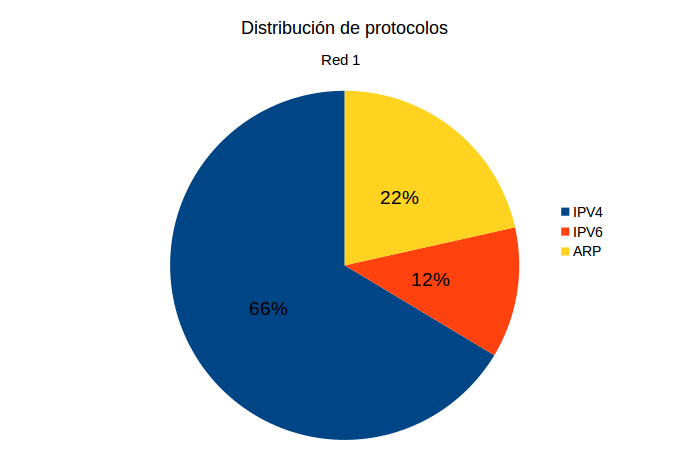
\includegraphics[scale=0.65]{imgs/red1_capturar.png}
	\caption{Distribución de protocolos de la red 1}
      \label{red1_capturar}
\end{figure}

Como podemos ver en la figura \ref{red1_capturar} hay un protocolo que tiene más presencia a la red: IPv4. Este protocolo es la piedra fundamental de la Internet, y es el que se usa para enviar paquetes de una red a otra a nivel mundial. IPv6 también se puede utilizar, pero todavía no tiene la suficiente adpoción como para reemplazar totalmente a IPv4, pero es una cuestión de tiempo ya que IPv4 está encontrando limitaciones técnicas que IPv6 soluciona. También aparecen en la red paquetes que usan el protocolo ARP descripto anteriormente que permite a los nodos de la red conocer la ubicación de otros nodos. Más adelante veremos el por qué de las apariciones de paquetes de protocolo ARP para esta red.

\begin{figure}[H]
	\centering
	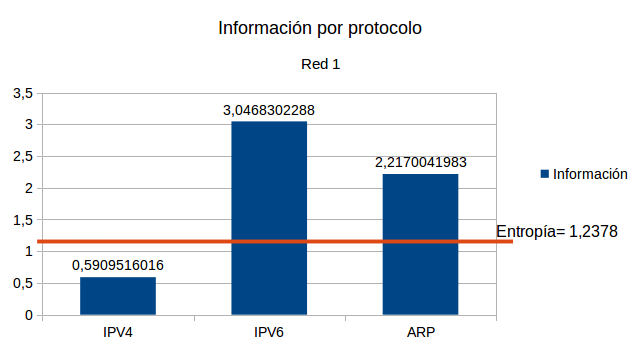
\includegraphics[scale=0.65]{imgs/red1_capturar_entropia.png}
	\caption{Cantidad de información que aporta cada protocolo, junto a la entropía de la fuente}
      \label{red1_capturar_entropia}
\end{figure}

Se puede apreciar en la figura \ref{red1_capturar_entropia} como vale la relación entre mayor cantidad de apariciones en la red implican un menor aporte de información. Asimismo vale la inversa, protocolos con pocas apariciones aportan mucha más información acerca de la fuente. La entropía viene a hacer el papel de un valor de información medio esperado por la fuente. Es decir, en cualquier momento se espera que la fuente arroje en promedio símbolos con información igual a la entropía. Un valor alto de entropía indicaría que estamos en presencia de una fuente de la cual no podemos decir con cierta seguridad qué símbolo emitirá la fuente. En este caso el protocolo IPv6 es el que más información debido a su baja frecuencia de aparición.

\subsubsection{Cafetería}

\begin{figure}[H]
	\centering
	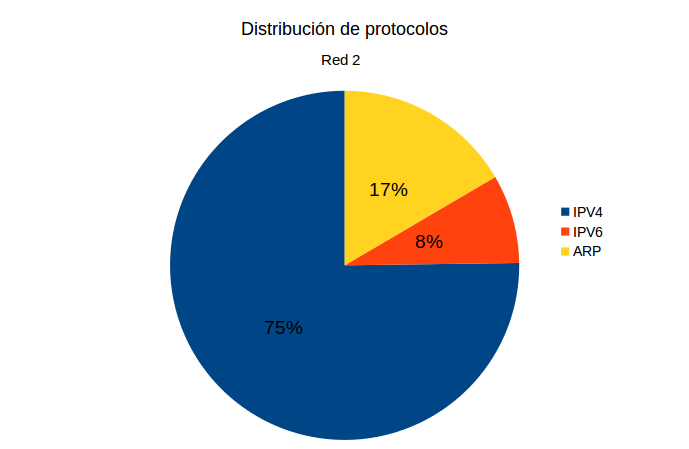
\includegraphics[scale=0.65]{imgs/red2_capturar.png}
	\caption{Distribución de protocolos de la red 2}
      \label{red2_capturar}
\end{figure}

Vemos ahora en la figura \ref{red2_capturar} que nuevamente IPv4 sobresale del resto en términos de frecuencia de aparición. Tiene sentido ya que esta red es una red de acceso público que suelen usarse principalmente para acceder a Internet para navegar o enviar o recibir mails o mensajes. Luego le siguen los paquetes del protocolo ARP, cuya frecuencia de aparición elevada se puede atribuir a que en una red de acceso público inalámbrica es común que constantemente se vayan agregando o retirando nodos de la red. Cada vez que un dispositivo nuevo se conecta a la red tiene que saber a qué nodo mandar los paquetes para poder acceder a Internet.

\begin{figure}[H]
	\centering
	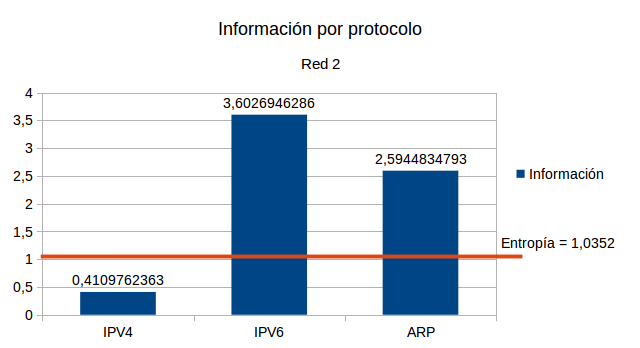
\includegraphics[scale=0.65]{imgs/red2_capturar_entropia.png}
	\caption{Cantidad de información que aporta cada protocolo, junto a la entropía de la fuente}
      \label{red2_capturar_entropia}
\end{figure}

En el caso de la figura \ref{red2_capturar_entropia} los paquetes con protocolo IPv6 son aún menos frecuentes que los anteriores ya que es una red de acceso público en la cuál se conecta toda variedad de dispositivos comerciales que sólo soportan el protocolo IPv4. Es por eso que la cantidad de información que aporta es muy alta. La entropía disminuye en medida de que un protocolo se vuelve cada vez más frecuente, como sucede en este caso en comparación a la red de la universidad.

\subsubsection{Ambientes laborales}

\begin{figure}[H]
	\centering
	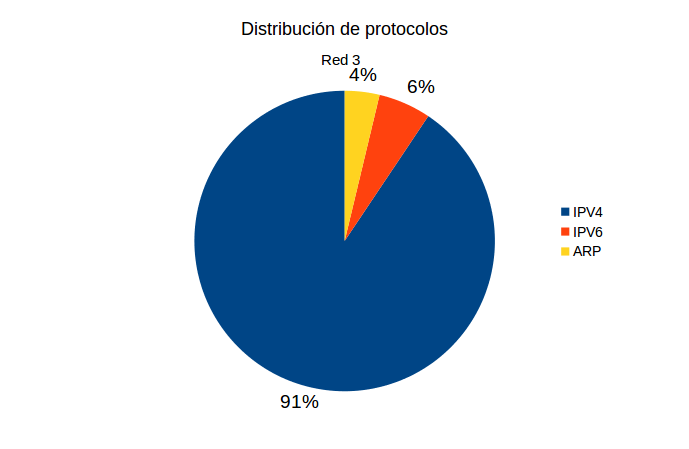
\includegraphics[scale=0.65]{imgs/red3_capturar.png}
	\caption{Distribución de protocolos de la red 3}
      \label{red3_capturar}
\end{figure}

\begin{figure}[H]
	\centering
	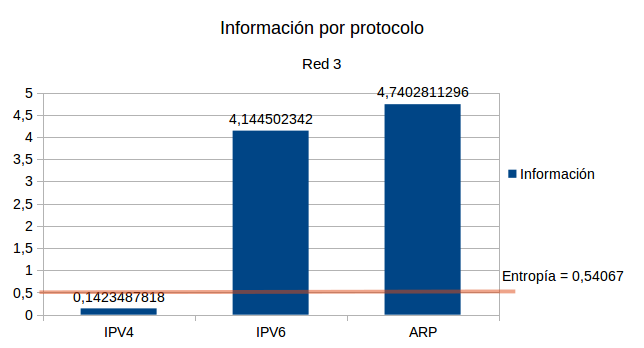
\includegraphics[scale=0.65]{imgs/red3_capturar_entropia.png}
	\caption{Cantidad de información que aporta cada protocolo, junto a la entropía de la fuente}
      \label{red3_capturar_entropia}
\end{figure}

\begin{figure}[H]
	\centering
	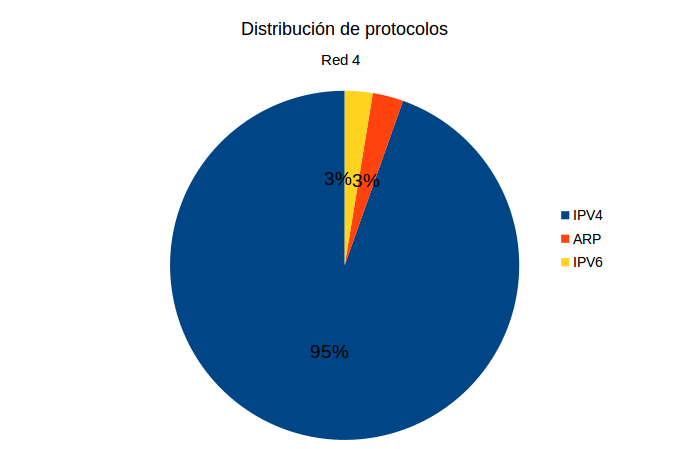
\includegraphics[scale=0.65]{imgs/red4_capturar.png}
	\caption{Distribución de protocolos de la red 4}
      \label{red4_capturar}
\end{figure}

\begin{figure}[H]
	\centering
	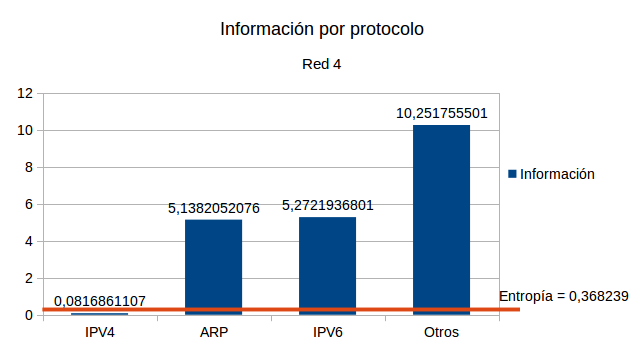
\includegraphics[scale=0.65]{imgs/red4_capturar_entropia.png}
	\caption{Cantidad de información que aporta cada protocolo, junto a la entropía de la fuente}
      \label{red4_capturar_entropia}
\end{figure}

Ahora vemos el caso de redes de ambientes laborales de las figuras \ref{red3_capturar} y \ref{red4_capturar} en donde se espera que sea estable en cantidad de nodos de que se conectan o desconectan a la red. En ambos casos el protocolo IPv4 es el más frecuente de todos y mucho más en comparación que las redes anteriores. Si los dispositivos se conectan a un servidor remoto en otra red (u otro país) es esperable ver muchos paquetes IP yendo a través de la red. 

También podemos observar tanto en la figura \ref{red3_capturar_entropia} y \ref{red4_capturar_entropia} que, al haber un protocolo tan frecuente, disminuye la entropía en comparación con las otras 2 redes anteriores. Asimismo aumenta la cantidad de información que aportan los protocolos IPv6 y ARP.


\newpage
\subsection{Experimento de identificación de nodos}

Veamos ahora el resultado de correr la herramienta \texttt{identificar.py} sobre las mismas capturas de las redes anteriores pero considerando a la fuente de información $S_1$ como aquella que emite direcciones de IP que aparecen como destino en los paquetes WHO\_HAS.

\subsubsection{Laboratorio de universidad}

\begin{figure}[H]
	\centering
	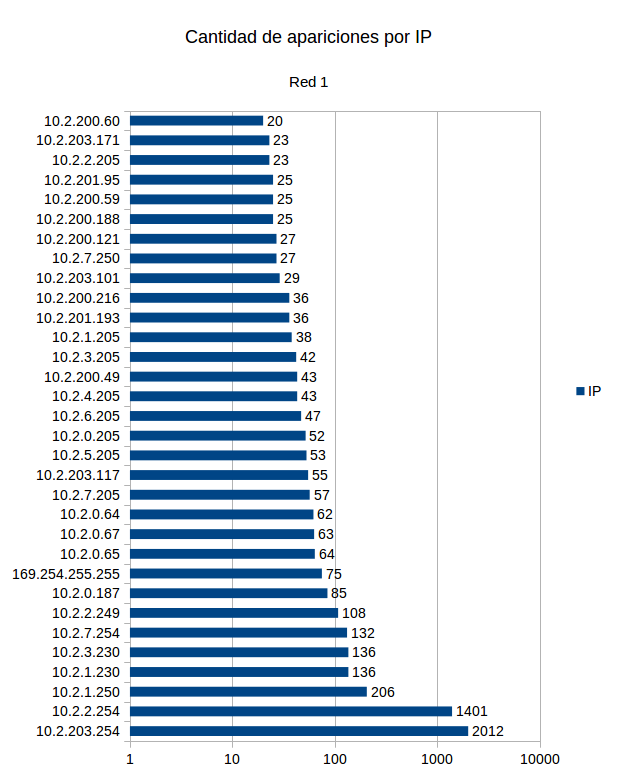
\includegraphics[scale=0.65]{imgs/red1_identificar.png}
	\caption{Cantidad de apariciones de direcciones IP en los paquetes ARP de la red 1}
      \label{red1_identificar}
\end{figure}

En la figura \ref{red1_identificar} podemos ver la cantidad de apariciones de cada dirección IP en los paquetes ARP de la red de la facultad. En realidad hay más direcciones IP en la lista, pero eran demasiadas para graficar, así que nos quedamos con las que más veces aparecen. Analizando la captura de los datos podemos ver que muchas de esas apariciones son de paquetes WHO\_HAS repetidos, donde un mismo nodo pregunta varias veces por esa IP. Esto es algo normal en una red WiFi porque es un medio poco confiable y suelen perderse los paquetes, más en una red con mucho tráfico. Esta es la razón también de porque la presencia de paquetes ARP en esta red era bastante grande, en comparación con otras redes. La cantidad de información que agregan paquetes repetidos claramente es baja, ya que más de un paquete no nos dice nada nuevo sobre la topología de la red.

\subsubsection{Cafetería}

\begin{figure}[H]
	\centering
	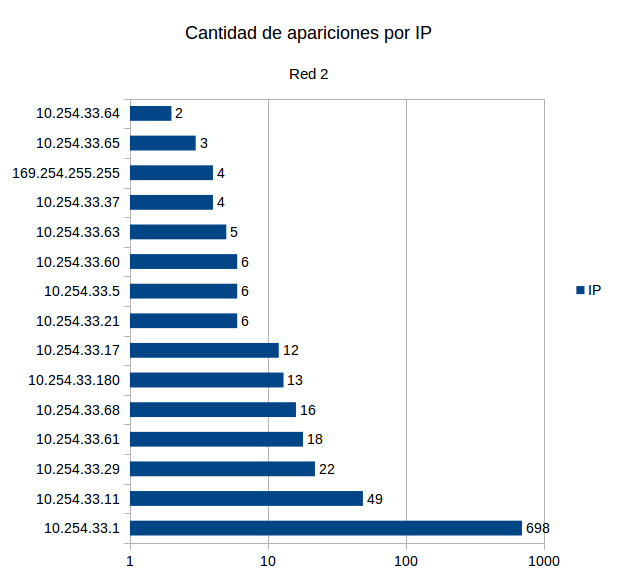
\includegraphics[scale=0.65]{imgs/red2_identificar.png}
	\caption{Cantidad de apariciones de direcciones IP en los paquetes ARP de la red 2}
      \label{red2_identificar}
\end{figure}

En un caso más normal, en la figura \ref{red2_identificar} podemos ver que el nodo con más apariciones es la primera dirección IP de la red \texttt{10.254.33.1\/24} que usualmente es el que se le asigna al router que se encargará de recibir y enviar paquetes entre la Internet y la red propiamente dicha. Un dispositivo cuando se conecta a la red WiFi necesita saber a qué dispositivo mandar los paquetes hacia Internet, así que realiza un envío de un paquete ARP preguntando por la dirección física de la IP \texttt{10.254.33.1}. Como los dispositivos en una cafetería van y vienen, es esperable la aparición de muchos de estos paquetes.

\subsubsection{Ambientes laborales}

\begin{figure}[H]
	\centering
	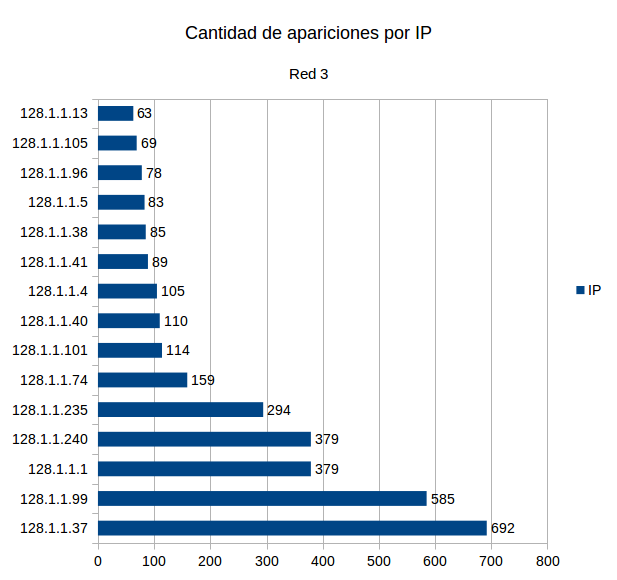
\includegraphics[scale=0.65]{imgs/red3_identificar.png}
	\caption{Cantidad de apariciones de direcciones IP en los paquetes ARP de la red 3}
      \label{red3_identificar}
\end{figure}

\begin{figure}[H]
	\centering
	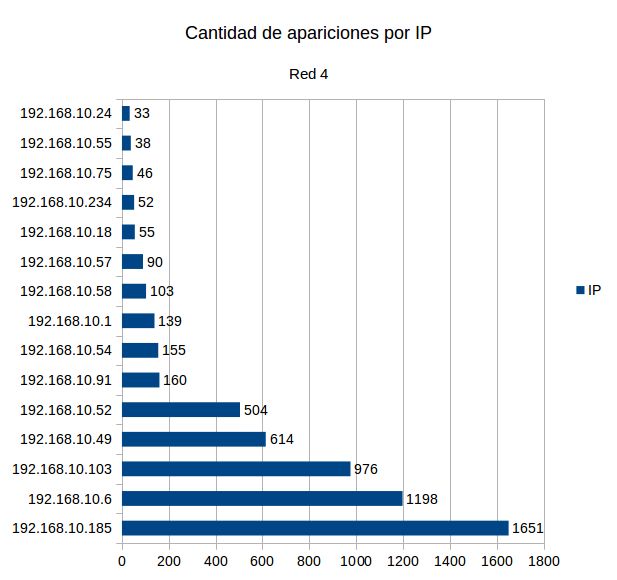
\includegraphics[scale=0.65]{imgs/red4_identificar.png}
	\caption{Cantidad de apariciones de direcciones IP en los paquetes ARP de la red 4}
      \label{red4_identificar}
\end{figure}

En las redes de ambientes de trabajo de las figuras \ref{red3_identificar} y \ref{red4_identificar} la dirección IP \texttt{128.1.1.1} no es la que más aparece, sino que hay otras. Posiblemente estas IP que más aparecen correspondan con nodos distinguidos en la red como un servidor, una base de datos, una impresora o algún otro recurso compartido por red.